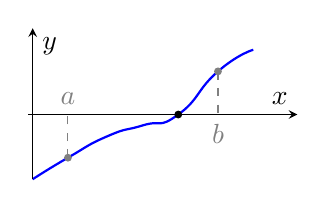
\begin{tikzpicture}
    \begin{axis}[
        axis lines = middle,
        axis on top,
        clip = false,
        xlabel = $x$,
        ylabel = {$y$},
        xtick = \empty,
        ytick = \empty,
        xmin=-0.1,xmax=6,
        ymin=-3,ymax=4,
        width=5cm,
        height=3.5cm
    ]
    
       % Define points0. , 0.8, 1.7, 2.5, 3.3, 4.2, 5. ]
    \coordinate (A) at (+0.0, -3.0);
    \coordinate (B) at (+0.8, -2.0);
    \coordinate (C) at (+1.7, -1.0);
    \coordinate (D) at (+2.5, -0.5);
    \coordinate (E) at (+3.3, +0.0);
    \coordinate (F) at (+4.2, +2.0);
    \coordinate (G) at (+5.0, +3.0);

    \coordinate (Ax) at (+0.0, +0.0);
    \coordinate (Bx) at (+0.8, +0.0);
    \coordinate (Cx) at (+1.7, +0.0);
    \coordinate (Dx) at (+2.5, -0.0);
    \coordinate (Ex) at (+3.3, +0.0);
    \coordinate (Fx) at (+4.2, +0.0);
    \coordinate (Gx) at (+5.0, +0.0);
    
    % Draw smooth curve through the points
    \draw [blue, thick] plot[smooth, tension=1] coordinates {(A) (B) (C) (D) (E) (F) (G)};
    
    % Draw points for reference
    \draw[gray, dashed] (B) node[circle, fill=gray, inner sep=1pt] {} -- (Bx)   node[at end, above] {$a$};
    \draw[gray, dashed] (F) node[circle, fill=gray, inner sep=1pt] {} -- (Fx)   node[at end, below] {$b$};
    
    \draw (E) node[circle, fill=black, inner sep=1pt] {};
    
    
    
    
    \end{axis}
    \end{tikzpicture}
